\section {Topics covered}
\begin{itemize}

\item Software quality

\item Software standards

\item Reviews and inspections

\item Software measurement and metrics

\end{itemize}
\section {Software quality management}
\begin{itemize}

\item Concerned with ensuring that the required level of quality is achieved in a software product.

\item Three principal concerns:

  \item At the organizational level, quality management is concerned with establishing a framework of organizational processes and standards that will lead to high-quality software.
  \item At the project level, quality management involves the application of specific quality processes and checking that these planned processes have been followed.
  \item At the project level, quality management is also concerned with establishing a quality plan for a project. The quality plan should set out the quality goals for the project and define what processes and standards are to be used.

\end{itemize}
\section {Quality management activities}
\begin{itemize}




\item Quality management provides an independent check on the software development process.

\item The quality management process checks the project deliverables to ensure that they are consistent with organizational standards and goals

\item The quality team should be independent from the development team so that they can take an objective view of the software. This allows them to report on software quality without being influenced by software development issues.

\end{itemize}

\section {Quality management and software development}
\begin{figure}[h!]
    \centering
    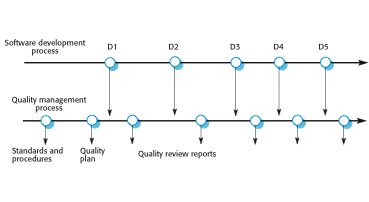
\includegraphics[width = 0.8\textwidth]{./figures/L7_1.png}
    \caption{}
    \label{fig:L7_1}
\end{figure}






\section {Quality planning}
\begin{itemize}
\item A quality plan sets out the desired product qualities and how these are assessed and defines the most significant quality attributes.

\item The quality plan should define the quality assessment process.

\item It should set out which organisational standards should be applied and, where necessary, define new standards to be used.
\end{itemize}


\section {Quality plans}
\begin{itemize}

\item Quality plan structure   \item Product introduction;   \item Product plans;   \item Process descriptions;   \item Quality goals;
  \item Risks and risk management.

\item Quality plans should be short, succinct documents   \item If they are too long, no-one will read them.
\end{itemize}

\section {Scope of quality management}
\begin{itemize}
\item Quality management is particularly important for large, complex systems. The quality documentation is a record of progress and supports continuity of development as the development team changes.

\item For smaller systems, quality management needs less documentation and should focus on establishing a quality culture.
\end{itemize}

\section {Software quality}
\begin{itemize}
\item Quality, simplistically, means that a product should meet its specification.

\item This is problematical for software systems

  \item There is a tension between customer quality requirements (efficiency, reliability, etc.) and developer quality requirements (maintainability, reusability, etc.);
  \item Some quality requirements are difficult to specify in an unambiguous way;
  \item Software specifications are usually incomplete and often inconsistent.

\item The focus may be ‘fitness for purpose’ rather than specification conformance.

\end{itemize}

\section {Software fitness for purpose}
\begin{itemize}

\item Have programming and documentation standards been followed in the development process?

\item Has the software been properly tested?

\item Is the software sufficiently dependable to be put into use?

\item Is the performance of the software acceptable for normal use?

\item Is the software usable?

\item Is the software well-structured and understandable?
\end{itemize}

\section {Software quality attributes}
\begin{table}[h!]
\centering
\begin{tabular}{ |p{3cm}|p{3cm}|p{3cm}|  }
\hline
Safety & Understandability & Portability\\
\hline
Security & Testability & Usability \\
\hline
Reliability & Adaptability & Reusability \\
\hline
Resilience & Modularity & Efficiency \\
\hline
Robustness & Complexity & Learnability\\
\hline
\end{tabular}

\label{table:T7_1}
\end{table}

\section {Quality conflicts}
\begin{itemize}

\item It is not possible for any system to be optimized for all of these attributes – for example, improving robustness may lead to loss of performance.

\item The quality plan should therefore define the most important quality attributes for the software that is being developed.

\item The plan should also include a definition of the quality assessment process, an agreed way of assessing whether some quality, such as maintainability or robustness, is present in the product.

\end{itemize} \section {Process and product quality}
\begin{itemize}

\item The quality of a developed product is influenced by the quality of the production process.

\item This is important in software development as some product quality attributes are hard to assess.

\item However, there is a very complex and poorly understood relationship between software processes and product quality.

  \item The application of individual skills and experience is particularly important in software development;
  \item External factors such as the novelty of an application or the need for an accelerated development schedule may impair product quality.
\end{itemize}
\section {Process-based quality}
\begin{figure}[h!]
    \centering
    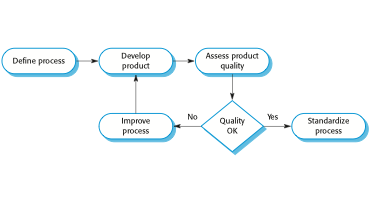
\includegraphics[width = 0.8\textwidth]{./figures/L7_2.png}
    \caption{}
    \label{fig:L7_2}
\end{figure}

\section {Software standards}
\begin{itemize}

\item Standards define the required attributes of a product or process. They play an important role in quality management.

\item Standards may be international, national, organizational or project standards.

\item Product standards define characteristics that all software components should exhibit e.g. a common programming style.

\item Process standards define how the software process should be enacted.
\end{itemize}
\section {Importance of standards}
\begin{itemize}


\item Encapsulation of best practice- avoids repetition of past mistakes.

\item They are a framework for defining what quality means in a particular setting i.e. that organization’s view of quality.

\item They provide continuity - new staff can understand the organisation by understanding the standards that are used.

\end{itemize}
\section {Product and process standards}
\begin{table}[h!]
\centering
\begin{tabular}{ |p{6cm}|p{6cm}|}
\hline
Product standards & Process standards\\
\hline
\hline
Design review form & Design review conduct\\
Requirements document structure & Submission of new code for system building\\
\hline
Method header format & Version release process\\
\hline
Java programming style & Project plan approval process\\
\hline
Project plan format & Change control process\\
\hline
Change request form & Test recording process\\
\hline
\end{tabular}

\label{table:T7_2}
\end{table}

\section {Problems with standards}
\begin{itemize}

\item They may not be seen as relevant and up-to-date by software engineers.

\item They often involve too much bureaucratic form filling.

\item If they are unsupported by software tools, tedious form filling work is often involved to maintain the documentation associated with the standards.


\end{itemize}
\section {Standards development}
\begin{itemize}
\item Involve practitioners in development. Engineers should understand the rationale underlying a standard.

\item Review standards and their usage regularly. Standards can quickly become outdated and this reduces their credibility amongst practitioners.

\item Detailed standards should have specialized tool support. Excessive clerical work is the most significant complaint against standards.

  \item Web-based forms are not good enough.
\end{itemize}
\section {ISO 9001 standards framework}
\begin{itemize}
\item An international set of standards that can be used as a basis for developing quality management systems.

\item ISO 9001, the most general of these standards, applies to organizations that design, develop and maintain products, including software.

\item The ISO 9001 standard is a framework for developing software standards.

  \item It sets out general quality principles, describes quality processes in general and lays out the organizational standards and procedures that should be defined. These should be documented in an organizational quality manual.

\end{itemize}
\section {ISO 9001 core processes}
\begin{figure}[h!]
    \centering
    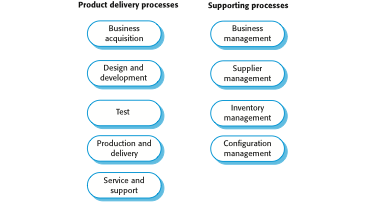
\includegraphics[width = 0.8\textwidth]{./figures/L7_3.png}
    \caption{}
    \label{fig:L7_3}
\end{figure}


\newpage
\section {ISO 9001 and quality management}
\begin{figure}[h!]
    \centering
    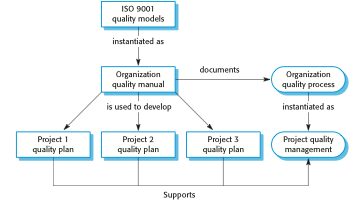
\includegraphics[width = 0.8\textwidth]{./figures/L7_4.png}
    \caption{}
    \label{fig:L7_4}
\end{figure}



\section {ISO 9001 certification}
\begin{itemize}
\item Quality standards and procedures should be documented in an organisational quality manual.
\item An external body may certify that an organisation’s quality manual conforms to ISO 9000 standards.
\item Some customers require suppliers to be ISO 9000 certified although the need for flexibility here is increasingly recognised.
\end{itemize}

\section {Key points}
\begin{itemize}
\item Software quality management is concerned with ensuring that software has a low number of defects and that it reaches the required standards of maintainability, reliability, portability and so on.

\item SQM includes defining standards for processes and products and establishing processes to check that these standards have been followed.

\item Software standards are important for quality assurance as they represent an identification of ‘best practice’.

\item Quality management procedures may be documented in an organizational quality manual, based on the generic model for a quality manual suggested in the ISO 9001 standard.
\end{itemize}
\section {Reviews and inspections}
\begin{itemize}

\item A group examines part or all of a process or system and its documentation to find potential problems.

\item Software or documents may be 'signed off' at a review which signifies that progress to the next development stage has been approved by management.

\item There are different types of review with different objectives

  \item Inspections for defect removal (product);

  \item Reviews for progress assessment (product and process);   \item Quality reviews (product and standards).
\end{itemize}
\section {Quality reviews}
\begin{itemize}

\item A group of people carefully examine part or all of a software system and its associated documentation.

\item Code, designs, specifications, test plans, standards, etc. can all be reviewed.

\item Software or documents may be 'signed off' at a review which signifies that progress to the next development stage has been approved by management.
\end{itemize}
\section {The software review process}
\begin{figure}[h!]
    \centering
    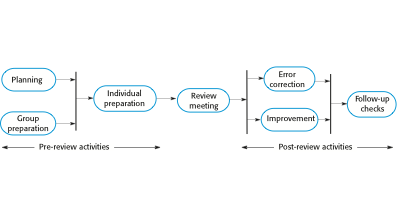
\includegraphics[width = 0.8\textwidth]{./figures/L7_5.png}
    \caption{}
    \label{fig:L7_5}
\end{figure}


\section {Reviews and agile methods}
\begin{itemize}

\item The review process in agile software development is usually informal.

  \item In Scrum, for example, there is a review meeting after each iteration of the software has been completed (a sprint review), where quality issues and problems may be discussed.

\item In extreme programming, pair programming ensures that code is constantly being examined and reviewed by another team member.

\item XP relies on individuals taking the initiative to improve and refactor code. Agile approaches are not usually standards-driven, so issues of standards compliance are not usually considered.

\item These are peer reviews where engineers examine the source of a system with the aim of discovering anomalies and defects.

\item Inspections do not require execution of a system so may be used before implementation.

\item They may be applied to any representation of the system (requirements, design,configuration data, test data, etc.).

\item They have been shown to be an effective technique for discovering program errors.

\end{itemize}
\section {Inspection checklists}
\begin{itemize}

\item Checklist of common errors should be used to drive the inspection.

\item Error checklists are programming language dependent and reflect the characteristic errors that are likely to arise in the language.

\item In general, the 'weaker' the type checking, the larger the checklist.

\item Examples: Initialisation, Constant naming, loop termination, array bounds, etc.
\end{itemize}
\newpage
\section {An inspection checklist}

\begin{longtable}{|p{2cm}|p{8cm}|}
% \centering
% \begin{tabular}{ |p{2cm}|p{8cm}|}
\hline
Fault class & Inspection check\\
\hline
\hline
Data faults &
\begin{itemize}
  	\item Are all program variables initialized before their values are used?
    \item Have all constants been named?
  	\item Should the upper bound of arrays be equal to the size of the array or Size -1?
  	\item If character strings are used, is a delimiter explicitly assigned?
    \item Is there any possibility of buffer overflow?
\end{itemize}\\
\hline
Control faults &
\begin{itemize}
  	\item For each conditional statement, is the condition correct?
    \item Is each loop certain to terminate?
  	\item Are compound statements correctly bracketed?
  	\item In case statements, are all possible cases accounted for?
  	\item If a break is required after each case in case statements, has it been included?
\end{itemize}\\
\hline
Input/output faults &
\begin{itemize}
  	\item Are all input variables used?
  	\item Are all output variables assigned a value before they are output?
    \item Can unexpected inputs cause corruption?
\end{itemize}\\
\hline
Interface faults &
\begin{itemize}
  	\item Do all function and method calls have the correct number of parameters?
  	\item Do formal and actual parameter types match?
    \item Are the parameters in the right order?
  	\item If components access shared memory, do they have the same model of the shared memory structure?
\end{itemize}\\
\hline
Storage	management faults &
\begin{itemize}
  	\item If a linked structure is modified, have all links been correctly reassigned?
  	\item If dynamic storage is used, has space been allocated correctly?
  	\item Is space explicitly deallocated after it is no longer required?
\end{itemize}\\
\hline
Exception	management faults &
\begin{itemize}
  	\item Have all possible error conditions been taken into account?
\end{itemize}\\
\hline
% \end{tabular}
\caption{}
\label{table:T7_3}
\end{longtable}

% \newpage
\section {Agile methods and inspections}
\begin{itemize}

\item Agile processes rarely use formal inspection or peer review processes.

\item Rather, they rely on team members cooperating to check each other’s code, and informal guidelines, such as ‘check before check-in’, which suggest that programmers should check their own code.

\item Extreme programming practitioners argue that pair programming is an effective substitute for inspection as this is, in effect, a continual inspection process.

\item Two people look at every line of code and check it before it is accepted.

\end{itemize}
\section {Software measurement and metrics}
\begin{itemize}
\item Software measurement is concerned with deriving a numeric value for an attribute of a software product or process.

\item This allows for objective comparisons between techniques and processes.

\item Although some companies have introduced measurement programmes, most organisations still don’t make systematic use of software measurement.

\item There are few established standards in this area.

\end{itemize}
\section {Software metric}
\begin{itemize}

\item Any type of measurement which relates to a software system, process or related documentation

  \item Lines of code in a program, the Fog index, number of person-days required to develop a component.

\item Allow the software and the software process to be quantified.

\item May be used to predict product attributes or to control the software process.

\item Product metrics can be used for general predictions or to identify anomalous components.
\end{itemize}
\section {Predictor and control measurements}
\begin{figure}[h!]
    \centering
    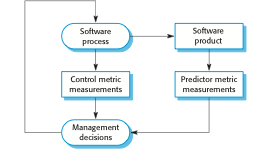
\includegraphics[width = 0.8\textwidth]{./figures/L7_6.png}
    \caption{}
    \label{fig:L7_6}
\end{figure}


\section {Use of measurements}
\begin{itemize}

\item To assign a value to system quality attributes

  \item By measuring the characteristics of system components, such as their cyclomatic complexity, and then aggregating these measurements, you can assess system quality attributes, such as maintainability.

\item To identify the system components whose quality is sub-standard

  \item Measurements can identify individual components with characteristics that deviate from the norm. For example, you can measure components to discover those with the highest complexity. These are most likely to contain bugs because the complexity makes them harder to understand.

\end{itemize}
\section {Metrics assumptions}
\begin{itemize}

\item A software property can be measured.

\item The relationship exists between what we can measure and what we want to know. We can only
measure internal attributes but are often more interested in external software attributes.

\item This relationship has been formalised and validated.

\item It may be difficult to relate what can be measured to desirable external quality attributes.
\end{itemize}
\newpage
\section {Relationships between internal and external software}
\begin{figure}[h!]
    \centering
    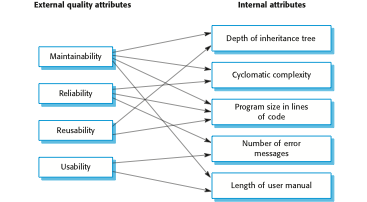
\includegraphics[width = 0.8\textwidth]{./figures/L7_7.png}
    \caption{}
    \label{fig:L7_7}
\end{figure}


\section {Problems with measurement in industry}
\begin{itemize}

\item It is impossible to quantify the return on investment of introducing an organizational metrics program.

\item There are no standards for software metrics or standardized processes for measurement and analysis.

\item In many companies, software processes are not standardized and are poorly defined and controlled.

\item Most work on software measurement has focused on code-based metrics and plan-driven development processes. However, more and more software is now developed by configuring ERP systems or COTS.

\item Introducing measurement adds additional overhead to processes.

\end{itemize}
\section {Product metrics}
\begin{itemize}

\item A quality metric should be a predictor of product quality.

\item Classes of product metric

  \item Dynamic metrics which are collected by measurements made of a program in execution;
  \item Static metrics which are collected by measurements made of the system representations;
  \item Dynamic metrics help assess efficiency and reliability

  \item Static metrics help assess complexity, understandability and maintainability.


\end{itemize}
\section {Dynamic and static metrics}
\begin{itemize}

\item Dynamic metrics are closely related to software quality attributes

  \item It is relatively easy to measure the response time of a system (performance attribute) or the number of failures (reliability attribute).

\item Static metrics have an indirect relationship with quality attributes

  \item You need to try and derive a relationship between these metrics and properties such as complexity, understandability and maintainability.
\end{itemize}

\newpage
\section {Static software product metrics}
\begin{table}[h!]
\centering
\begin{tabular}{ |p{3cm}|p{8cm}| }
\hline
Software metric & Description\\
\hline
\hline
Fan-in/Fan-out & Fan-in is a measure of the number of functions or methods that call another function or method (say X). Fan-out is the number of functions that are called by function X. A high value for fan-in means that X is tightly coupled to the rest of the design and changes to X will have extensive knock-on effects. A high value for fan-out suggests that the overall complexity of X may be high because of the complexity of the control logic needed to coordinate the called components.\\
\hline
Length of code & This is a measure of the size of a program. Generally, the larger the size of the code of a component, the more complex and error-prone that component is likely to be. Length of code has been shown to be one of the most reliable	metrics	for	predicting	error-proneness	in components.\\
\hline
Cyclomatic complexity & This is a measure of the control complexity of a program. This control complexity may be related to program understandability. I discuss cyclomatic complexity in Chapter 8.\\
\hline
Length of identifiers & This is a measure of the average length of identifiers (names for variables, classes, methods, etc.) in a program. The longer the identifiers, the more likely they are	to	be	meaningful	and	hence	the	more understandable the program.\\
\hline
Depth of conditional nesting & This is a measure of the depth of nesting of if-statements in a program. Deeply nested if-statements are hard to understand and potentially error-prone.\\
\hline
Fog index & This is a measure of the average length of words and sentences in documents. The higher the value of a document’s Fog index, the more difficult the document is to understand.\\
\hline
\end{tabular}

\label{table:T7_4}
\end{table}

\section {Software component analysis}
\begin{itemize}

\item System component can be analyzed separately using a range of metrics.

\item The values of these metrics may then compared for different components and, perhaps, with historical measurement data collected on previous projects.

\item Anomalous measurements, which deviate significantly from the norm, may imply that there are problems with the quality of these components.


\end{itemize}
\section {The process of product measurement}
\begin{figure}[h!]
    \centering
    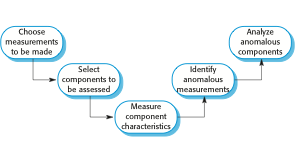
\includegraphics[width = 0.8\textwidth]{./figures/L7_8.png}
    \caption{}
    \label{fig:L7_8}
\end{figure}



\section {Measurement surprises}
\begin{itemize}
\item Reducing the number of faults in a program leads to an increased number of help desk calls

  \item The program is now thought of as more reliable and so has a wider more diverse market. The percentage of users who call the help desk may have decreased but the total may increase;
  \item A more reliable system is used in a different way from a system where users work around the faults. This leads to more help desk calls.

\end{itemize}

\section {Key points}
\begin{itemize}


\item Reviews of the software process deliverables involve a team of people who check that quality standards are being followed.

\item In a program inspection or peer review, a small team systematically checks the code. They read the code in detail and look for possible errors and omissions

\item Software measurement can be used to gather data about software and software processes.

\item Product quality metrics are particularly useful for highlighting anomalous components that may have quality problems.
\end{itemize}


\section {The CK object-oriented metrics suite}
\begin{table}[h!]
\centering
\begin{tabular}{ |p{3cm}|p{8cm}| }
  \hline
Object-oriented metric & Description\\
\hline
\hline
Weighted methods per class (WMC) & This is the number of methods in each class, weighted by the complexity of each method. Therefore, a simple method may have a complexity of 1, and a large and complex method a much higher value. The larger the value for this metric, the more complex the object class. Complex objects are more likely to be difficult to understand. They may not be logically cohesive, so cannot be reused effectively as superclasses in an inheritance tree.\\
\hline
Depth of inheritance tree (DIT) & This represents the number of discrete levels in the inheritance tree where subclasses inherit attributes and operations (methods) from superclasses. The deeper the inheritance tree, the more complex the design. Many object classes may have to be understood to understand the object classes at the leaves of the tree.\\
\hline
Number of children (NOC) & This is a measure of the number of immediate subclasses in a class. It measures the breadth of a class hierarchy, whereas DIT measures its depth. A high value for NOC may indicate greater reuse. It may mean that more effort should be made in validating base classes because of the number of subclasses that depend on them.\\
\hline
Coupling between object classes (CBO) & Classes are coupled when methods in one class use methods or instance variables defined in a different class. CBO is a measure of how much coupling exists. A high value for CBO means that classes are highly dependent, and therefore it is more likely that changing one class will affect other classes in the program.\\
\hline
Response for a class (RFC) & RFC is a measure of the number of methods that could potentially be executed in response to a message received by an object of that class. Again, RFC is related to complexity. The higher the value for RFC, the more complex a class and hence the more likely it is that it will include errors.\\
\hline
Lack of cohesion in methods (LCOM) & LCOM is calculated by considering pairs of methods in a class. LCOM is the difference between the number of method pairs without shared attributes and the number of method pairs with shared attributes. The value of this metric has been widely debated and it exists in several variations. It is not clear if it really adds any additional, useful information over and above that provided by other metrics.\\
\hline
\end{tabular}

\label{table:T7_5}
\end{table}
